\chapter{Použité technologie, techniky, pojmy}
\section{GitHub}
Github je~online platforma, která umožňuje vývojářům ukládat a~sdílet jejich kód. Na~githubu je~kód ukládán v~repozitářích. V~repozitářích je~kromě samotného kódu uložena i~historie změn.

Jakýkoliv jiný uživatel si~může z~githubu stáhnout repozitář, pozměnit ho~a~následně autorovi navrhnout začlenění jeho změn do~původního repozitáře.

Celá výsledná softwarová výbava projektoru byla nahrána na~server github.com do~repozitáře \href{https://github.com/phuid/laser_projector}{phuid/laser\_projector}. Do~tohoto repozitáře budou nahrány i~jakékoliv pozdější změny softwarové výbavy.

\section{Node.js}
Node.js je~open-source runtime (česky běhové prostředí) pro~javascript, které umožňuje vývojářům spouštět javascriptový kód mimo prohlížeč~\cite{nodejs-wiki}.
Umožňuje tedy programovat kód pro~server ve~stejném jazyce, který běží v~prohlížeči. Díky tomu je~oblíbený mimo jiné pro~tvoření serverů hostujících webové stránky.

\section{SPI}\label{sec:spi}
SPI (anglicky Serial Peripheral Interface) je~komunikační rozhraní používané k~přenosu dat~mezi ovládajícím zařízením (často mikrokontrolerem) a~jedním, nebo více periferními integrovynými obvody (periferiemi).
Používá separátní vodič (linky) pro~hodinový signál (SCK), kterým mikrokontroler ovládá rychlost přenosu dat, a~datové linky.
Datové linky jsou fixně využívané k~posílání dat~buď periferií -- linka POCI (Peripheral Out, Controller In), nebo mikrokontrolerem -- linka PICO (Peripheral In, Controller Out).
Dále používá separátní vodič(e) pro~výběr periferie, se~kterou mikrokontroler komunikuje. Tomuto vodiči se~říká chip select (zkráceně CS). Pro~každou periferii je~potřeba připojit separátní CS~vodič.~\cite{sparkfun-spi}

\section{I$^{2}$C}
I$^{2}$C (anglicky Inter-Integrated Circuit) je~komunikační protokol umožňující komunikaci mezi jednou nebo více periferiemi a~jedním, nebo více mikrokontrolery.
Podobně jako SPI~je~úrčen ke~komunikaci na~krátké vzdálenosti v~jednom zařízení.
Narozdíl od~SPI~využívá pouze dva~vodiče (zvané SDA~a SCL) k~výměně informací včetně výběru připojené periferie, se~kterou mikrokontroler chce komunikovat.
Zároveň umožňuje fungování systémů s~několika kontrolery.~\cite{sparkfun-i2c}

Dva vodiče při použití tohoto protokolu stačí i~na~výběr zařízení, se~kterým chce mikrokontroler komunikovat.
Po začátku komunikace totiž sběrnicí\footnote{Sběrnice I$^{2}$C je~systém zařízení propojený protokolem I$^{2}$C na~dvou stejných vodičích.} mikrokontroler pošle tzv. adresu zařízení, se~kterým chce komunikovat~\cite{sparkfun-i2c}.
Adresa zařízení je~sestavena ze~sedmi bitů a~může tedy dosahovat 127 různých hodnot (kromě systémů s~10bitovou adresou; Ty~jsou ale~vzácné).
Většinou je~pro~danou periferii nastavena od~výroby, u~některých je~ale~možné ji~softwarově změnit.

% \section{Pull-up a~pull-down rezistory}
% \fxnote{possibly zbytecne TODO: oddelat}
% Pokud při čtení z~GPIO pinů mikrokontrolerů či jiných zařízení k~danému pinu není nic~připojeno, je~těžké předpovědět, jaký stav na~tomto pinu přečteme.
% Když tento fenomén nastane, říká se, že je~pin~floating (plovoucí)~\cite{sparkfun-pud}.
% Může nastat například, chceme-li číst stav tlačítka, přes které by~byl~pin připojen na~zem. Když tlačítko není zmáčknuté, pin~na~zem~připojen není a~tudíž je~floating.

% V takových případech se~k~pinu připojuje tzv. pull-up rezistor, který zaručí, že z~pinu v~případě, že tlačítko stisknuté není, přečteme hodnotu HIGH.
% Rozdíl mezi pull-up a~pull-down rezistory je~pouze v~tom, že pull-up rezistory připojují pin~k napětí, na~kterém zařízení pracuje (často 3,3 nebo 5~V) a~pull-down rezistory rezistory připojují pin~k zemi.~\cite{sparkfun-pud}

\section{PWM (Pulse Width Modulation)}\label{sec:pwm}
PWM (z~anglického Pulse Width Modulation) se~využívá jako alternativa analogového řízení v~případech, kdy~je~potřeba řídit analogovou proměnnou binárním signálem, tedy signálem nabývyjících hodnot \uv{zapnuto/vypnuto}.
V PWM~signálu je~konstantní perioda a~proměnný je~čas, kdy~má binární signál hodnotu \uv{zapnuto}, tomuto času se~říká \uv{pulse width} a~vyplývá z~něj jméno techniky. Konečná hodnota (\uv{střída}, anglicky \uv{duty cycle}) signálu se~dá získat jako poměr času \uv{pulse width} a~periody signálu.
Střída hodnoty 100~\% tedy znamená, že signál má neustále hodnotu \uv{zapnuto}, střída hodnoty 0~\% naopak znamená neustálé \uv{vypnuto}.~\cite{pwm}\cite{wiki_pwm}

Výsledný signál při využití této techniky je~ilustrován na~obrázku~\ref{fig:pwm}. V~reálném využití bývá frekvence PWM~signálu v~řádech kHz.

\begin{figure}[htb]
  \centering
  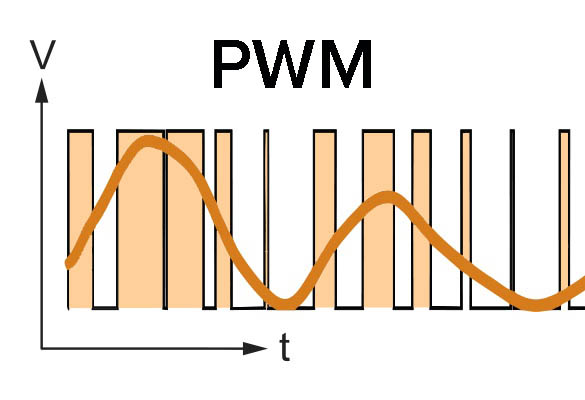
\includegraphics[width=0.4\textwidth]{img/pwm.jpg}
  \caption{\label{fig:pwm} PWM~signál s~měnící se~střídou; Střída naznačena oranžovou křivkou. Převzato a~upraveno z~\cite{pwm-image}}
\end{figure}

\section{Přerušení (Interrupt)}
Přerušení nastává, nastane-li za běhu programu náhle potřeba obsloužit hardwarovou událost. Procesor při něm přeruší vykonávání sledu instrukcí, obslouží přerušení a poté pokračuje v předchozí činnosti~\cite{wiki-interrupt}.
